\documentclass[10pt]{beamer}

\usetheme{CambridgeUS}
%\usecolortheme{beaver}

\definecolor{darkcyan}{RGB}{0,128,128}
\definecolor{lightcyan}{RGB}{204,238,238}
\definecolor{mediumcyan}{RGB}{0,153,153}

\setbeamercolor{palette primary}{bg=lightcyan,fg=black}
\setbeamercolor{palette secondary}{bg=mediumcyan,fg=white}
\setbeamercolor{palette tertiary}{bg=darkcyan,fg=white}
\setbeamercolor{palette quaternary}{bg=darkcyan!80,fg=white}

\setbeamercolor{structure}{fg=darkcyan}
\setbeamercolor{titlelike}{parent=palette tertiary}

\setbeamercolor{block title}{bg=darkcyan,fg=white}
\setbeamercolor{block body}{bg=lightcyan,fg=black}

\setbeamercolor{author in head/foot}{bg=darkcyan!90,fg=white}
\setbeamercolor{title in head/foot}{bg=darkcyan!70,fg=white}

\usepackage[utf8]{inputenc}
\usepackage[T1]{fontenc}
\usepackage{booktabs}
\usepackage{multirow}
\usepackage{textcomp}
\usepackage{listings}
\usepackage{xcolor}
\usepackage{tikz}
\usetikzlibrary{shapes,arrows,positioning,fit,calc}

\setbeamertemplate{navigation symbols}{}

\setbeamertemplate{footline}{
    \leavevmode
    \hbox{\begin{beamercolorbox}[wd=.35\paperwidth,ht=2.5ex,dp=1.25ex,center]{author in head/foot}
        \usebeamerfont{author in head/foot}\insertinstitute
    \end{beamercolorbox}
    \begin{beamercolorbox}[wd=.35\paperwidth,ht=2.5ex,dp=1.25ex,center]{author in head/foot}
        \usebeamerfont{author in head/foot}\insertshorttitle
    \end{beamercolorbox}
    \begin{beamercolorbox}[wd=.30\paperwidth,ht=2.5ex,dp=1.25ex,center]{author in head/foot}
        \usebeamerfont{author in head/foot}\insertframenumber\,/\,\inserttotalframenumber
    \end{beamercolorbox}}
    \vskip0pt
}

\lstset{
    basicstyle=\ttfamily\footnotesize,
    breaklines=true,
    frame=single,
    backgroundcolor=\color{gray!10}
}

\title[Smart Pharmacy]{STM32 Smart Pharmacy}
\subtitle{Bare-Metal Medication Dispenser on STM32F103C8T6}
\author{Khaled Mahfouz + Bilal Almaraashli}
\institute{Damascus University CAE}
\date{\today}

\begin{document}

\begin{frame}
    \titlepage
\end{frame}

\begin{frame}{Project Idea}
    \textbf{Problem:} Manual medication management is error-prone --- missed doses,
    incorrect timing, lack of monitoring.

    \vfill
    \textbf{Solution:} An embedded medication dispenser that:
    \begin{itemize}
        \item Controls two independent timed compartments
        \item Requires a 4-digit PIN to open (\emph{child-safe})
        \item Monitors ambient temperature and humidity
        \item Provides visual \emph{and} audible alerts
    \end{itemize}

    \vfill
    \centering
    \emph{No CubeIDE --- pure CMake, GCC, OpenOCD, and GDB.}
\end{frame}

\begin{frame}{System Block Diagram}
    \centering
    \small
    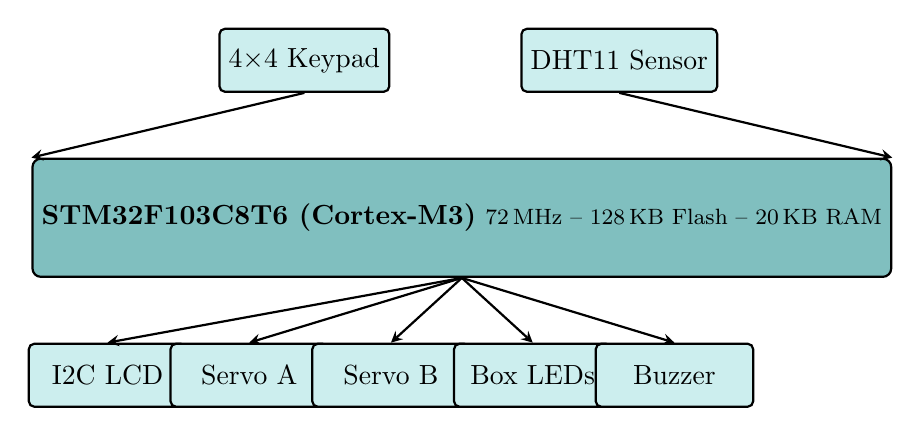
\begin{tikzpicture}[
        comp/.style={draw,fill=lightcyan,thick,minimum width=2cm,minimum height=0.8cm,rounded corners=2pt},
        mcu/.style={draw,fill=darkcyan!50,thick,minimum width=5cm,minimum height=1.5cm,rounded corners=3pt},
        arrow/.style={thick,->,>=stealth},
    ]

    \node[comp] (keypad) at (0,0) {4$\times$4 Keypad};
    \node[comp] (dht11)  at (4,0) {DHT11 Sensor};

    \node[mcu] (mcu) at (2,-2) {
        \textbf{STM32F103C8T6 (Cortex-M3)}\\[2pt]
        \footnotesize 72\,MHz -- 128\,KB Flash -- 20\,KB RAM
    };

    \node[comp] (lcd) at (-2.5,-4) {I2C LCD};
    \node[comp] (sv1) at (-0.7,-4) {Servo A};
    \node[comp] (sv2) at (1.1,-4)  {Servo B};
    \node[comp] (leds) at (2.9,-4) {Box LEDs};
    \node[comp] (buz)  at (4.7,-4) {Buzzer};

    \draw[arrow] (keypad.south) -- (mcu.north west);
    \draw[arrow] (dht11.south)  -- (mcu.north east);
    \draw[arrow] (mcu.south) -- (lcd.north);
    \draw[arrow] (mcu.south) -- (sv1.north);
    \draw[arrow] (mcu.south) -- (sv2.north);
    \draw[arrow] (mcu.south) -- (leds.north);
    \draw[arrow] (mcu.south) -- (buz.north);
    \end{tikzpicture}

    \vfill
    \small Resources: 128\,KB Flash, 20\,KB RAM \quad
    Clocks: HSE 8\,MHz $\rightarrow$ PLL $\rightarrow$ 72\,MHz
\end{frame}

\begin{frame}[fragile]{Software Overview}
    \textbf{Modular design --- each module does one thing:}

    \medskip
    \begin{columns}[t]
        \column{0.48\textwidth}
        \begin{itemize}
            \item \texttt{keypad.c} --- 4$\times$4 scan, debounce
            \item \texttt{servo.c} --- TIM3 PWM control
            \item \texttt{lcd.c} --- I2C HD44780 driver
            \item \texttt{dht11.c} --- single-wire protocol
            \item \texttt{buzzer.c} --- DWT-based tone gen.
        \end{itemize}

        \column{0.48\textwidth}
        \begin{itemize}
            \item \texttt{actuator.c} --- box LED control
            \item \texttt{state\_machine.c} --- app logic
            \item \texttt{error\_handler.c} --- fatal errors
            \item \texttt{delay.c} --- DWT microsecond delay
            \item \texttt{CMake + GCC + OpenOCD} --- toolchain
        \end{itemize}
    \end{columns}

    \vfill
    \begin{block}{Build \& Flash}
        \texttt{cmake -Bbuild \&\& cmake --build build \&\& cmake --build build --target flash}
    \end{block}

    \begin{block}{Debug}
        \texttt{openocd \ldots \&\& arm-none-eabi-gdb -x .gdbinit build/blink.elf}
    \end{block}
\end{frame}

\begin{frame}[fragile]{State Machine}
    \centering
    \footnotesize
    \begin{verbatim}
+----------+   +----------+   +----------+   +----------+
| PASSWORD |-->| TIMER_A  |-->| TIMER_B  |-->| MONITOR  |
|(4 digits)|   |(Box A s) |   |(Box B s) |   |(countdown)|
+----------+   +----------+   +----------+   +--+----+---+
                                                |    |
                                              A |    | B
                                                |    |
                                          +-----+    +-----+
                                          |                |
                                     +----v----+    +----v----+
                                     | ACTIVE_1|    | ACTIVE_2|
                                     |servo+LED|    |servo+LED|
                                     | PIN+*   |    | PIN+*   |
                                     |  close  |    |  close  |
                                     +----+----+    +----+----+
                                          |                |
                                          +-------+--------+
                                                  |
                                               +--v---+
                                               |LOOP  |
                                               |to M. |
                                               +-------+
    \end{verbatim}
\end{frame}

\begin{frame}{Lessons Learned}
    \begin{columns}[t]
        \column{0.48\textwidth}
        \textbf{Hardware lessons:}
        \begin{itemize}
            \item Always verify TIM channel mapping against
                  the MCU datasheet (PB0/1 = CH3/4, not CH1/2)
            \item Check pin conflicts early --- UART, DHT11,
                  and keypad all wanted PA2/PA3
            \item PC13 has an on-board pull-up resistor;
                  suitable for DHT11 data line
        \end{itemize}

        \vspace{8pt}
        \textbf{Protocol lessons:}
        \begin{itemize}
            \item PCF8574 I2C backpack for HD44780 LCD
                  needs correct nibble-split with enable
                  toggling --- most example code online is wrong
            \item DHT11 single-wire requires $\mu$s precision;
                  DWT cycle counter is the cleanest solution
        \end{itemize}

        \column{0.48\textwidth}
        \textbf{Software design lessons:}
        \begin{itemize}
            \item Data tables beat if/else chains ---
                  always prefer lookup tables over conditionals
            \item Each module should own its own
                  hardware resource definitions (pin, port, etc.)
            \item Shared utilities (like \texttt{delay.c})
                  eliminate code duplication
            \item Separate peripheral init from
                  business logic --- init in main.c,
                  state machine only handles transitions
        \end{itemize}

        \vspace{8pt}
        \textbf{Toolchain lessons:}
        \begin{itemize}
            \item Pure CMake + GCC + OpenOCD works
                  well and avoids vendor lock-in
            \item GDB debugging over ST-Link
                  is fast and reliable
        \end{itemize}
    \end{columns}
\end{frame}

\begin{frame}{Thank You}
    \centering
    \vfill
    {\Huge Questions?}
    \vfill
    \textbf{Repository:} \texttt{github.com/KhaledMahfouz5/stm32-without-cubeide}

    \medskip
    \textbf{Built with:}
    \begin{itemize}
        \item GCC \texttt{arm-none-eabi}, CMake, OpenOCD
        \item STM32CubeF1 HAL (submodule)
        \item ST-Link programmer
    \end{itemize}
    \vfill
\end{frame}

\end{document}

